\begin{figure}
    \centering

    \begin{subfigure}[t]{\textwidth}
        \centering
        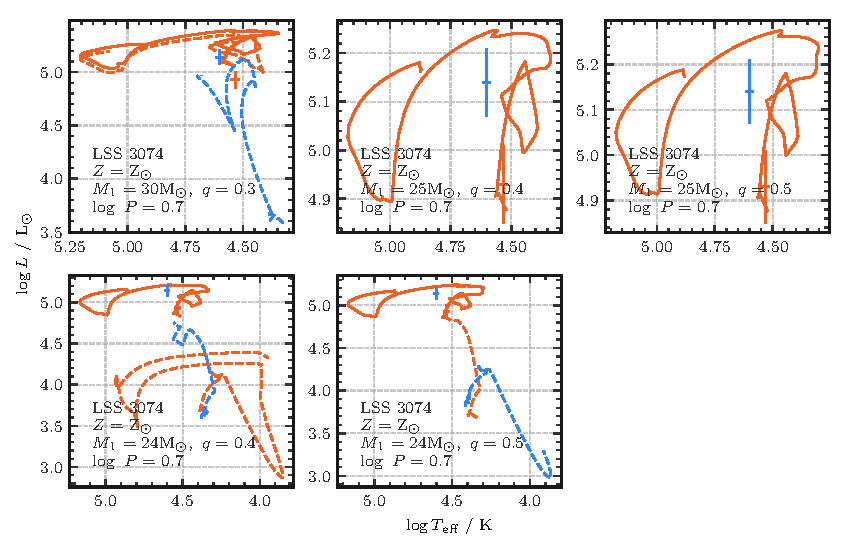
\includegraphics[width=\textwidth]{images/overcontact_binaries/bespoke_binaries/wider/LSS 3074.pdf}
        \caption{LSS 3074}
        \label{fig:bespoke_LSS_3074_wider}
    \end{subfigure}

    \begin{subfigure}[t]{\textwidth}
        \centering
        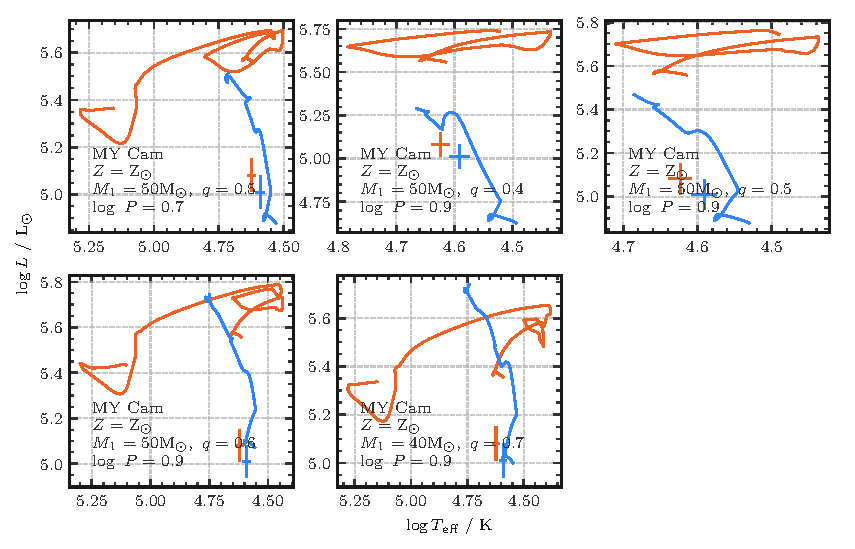
\includegraphics[width=\textwidth]{images/overcontact_binaries/bespoke_binaries/wider/MY Cam.pdf}
        \caption{MY Camelopardalis}
        \label{fig:bespoke_MY_Cam_wider}
    \end{subfigure}
\end{figure}%
\begin{figure}\ContinuedFloat
    \centering

    \begin{subfigure}[t]{\textwidth}
        \centering
        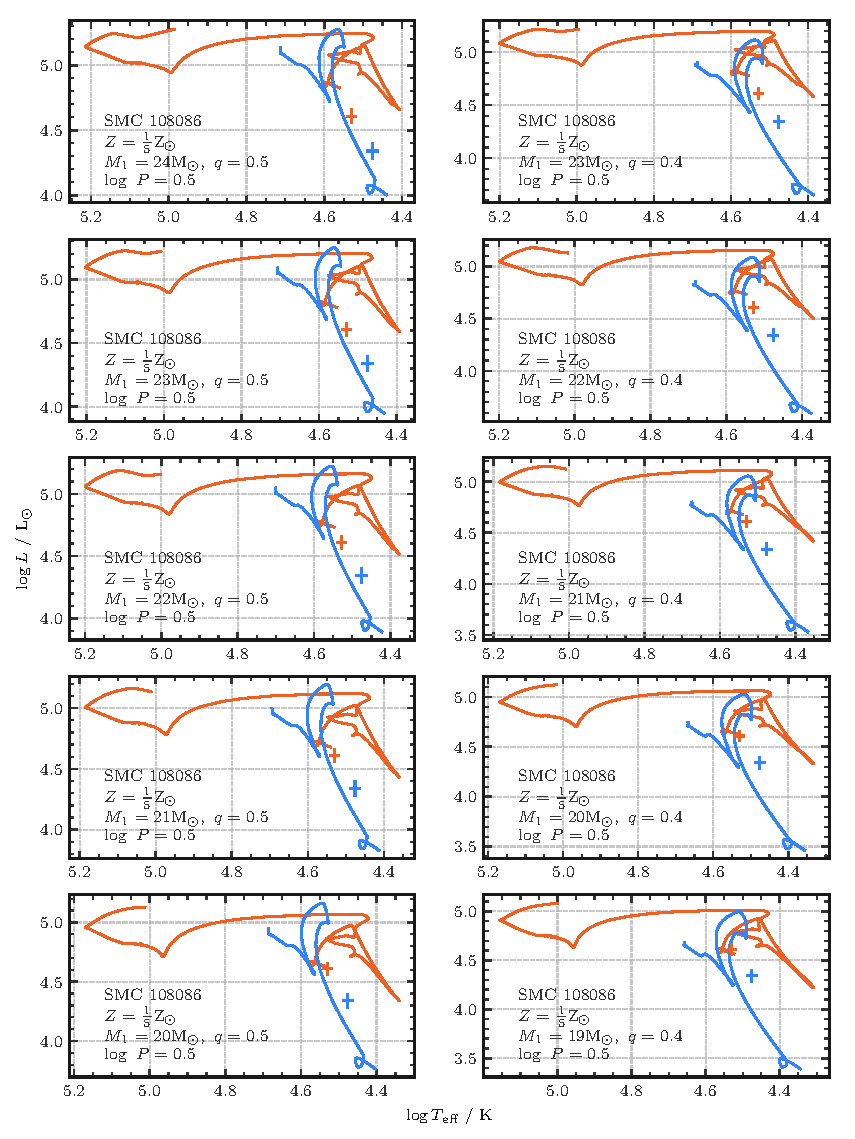
\includegraphics[width=\textwidth]{images/overcontact_binaries/bespoke_binaries/wider/SMC 108086.pdf}
        \caption{SMC 108086}
        \label{fig:bespoke_SMC_108086_wider}
    \end{subfigure}
\end{figure}%
\begin{figure}\ContinuedFloat
    \centering

    \begin{subfigure}[t]{\textwidth}
        \centering
        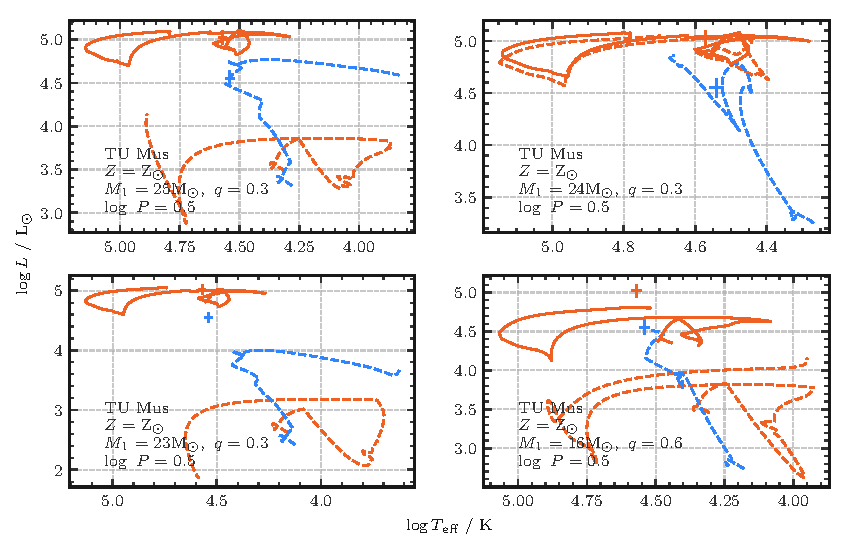
\includegraphics[width=\textwidth]{images/overcontact_binaries/bespoke_binaries/wider/TU Mus.pdf}
        \caption{TU Muscae}
        \label{fig:bespoke_TU_Mus_wider}
    \end{subfigure}

    \begin{subfigure}[t]{\textwidth}
        \centering
        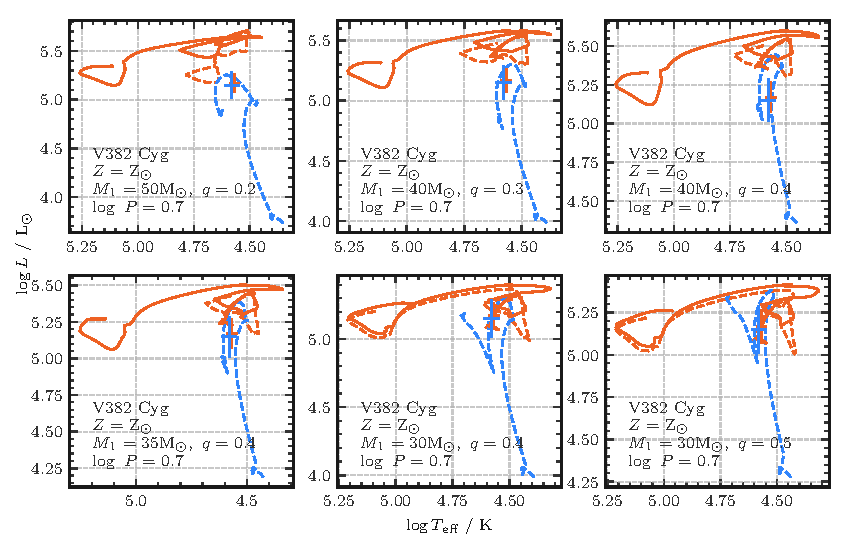
\includegraphics[width=\textwidth]{images/overcontact_binaries/bespoke_binaries/wider/V382 Cyg.pdf}
        \caption{V382 Cygni}
        \label{fig:bespoke_V382_Cyg_wider}
    \end{subfigure}

\end{figure}%
\begin{figure}\ContinuedFloat
    \centering

    \begin{subfigure}[t]{\textwidth}
        \centering
        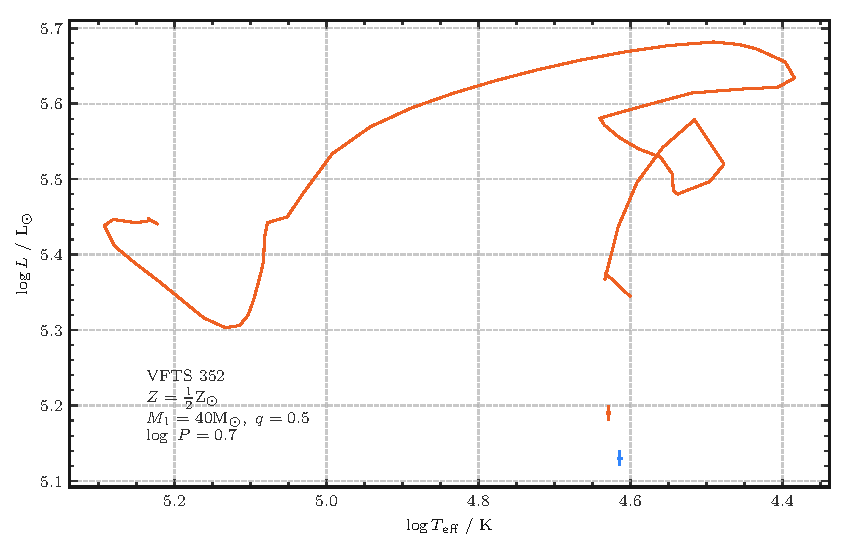
\includegraphics[width=\textwidth]{images/overcontact_binaries/bespoke_binaries/wider/VFTS 352.pdf}
        \caption{VFTS 352}
        \label{fig:bespoke_VFTS_352_wider}
    \end{subfigure}

    \caption[The results of our bespoke binary evolution for wider periods.]{The results of our bespoke binary evolution for \textbf{wider} periods. In these plots, orange lines represent the donors, and blue lines represent the accretors.}
    \label{fig:bespoke_binaries_wider}
\end{figure}

% NORMAL

\begin{figure}
    \centering

    \begin{subfigure}[t]{\textwidth}
        \centering
        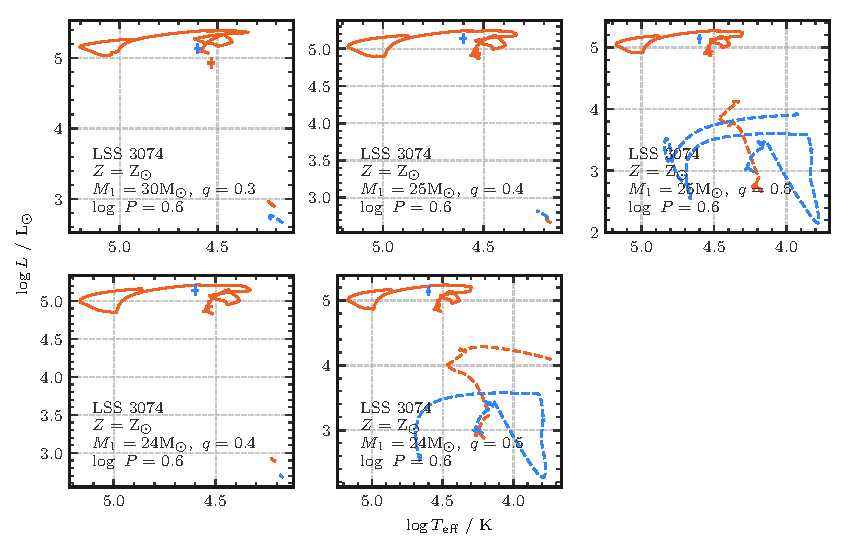
\includegraphics[width=\textwidth]{images/overcontact_binaries/bespoke_binaries/normal/LSS 3074.pdf}
        \caption{LSS 3074}
        \label{fig:bespoke_normal_LSS_3074}
    \end{subfigure}

    \begin{subfigure}[t]{\textwidth}
        \centering
        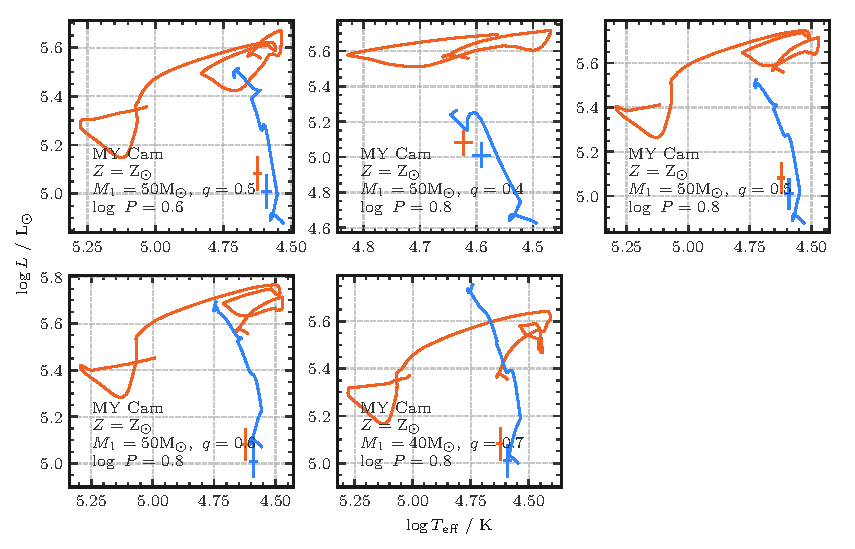
\includegraphics[width=\textwidth]{images/overcontact_binaries/bespoke_binaries/normal/MY Cam.pdf}
        \caption{MY Camelopardalis}
        \label{fig:bespoke_MY_Cam_normal}
    \end{subfigure}
\end{figure}%
\begin{figure}\ContinuedFloat
    \centering

    \begin{subfigure}[t]{\textwidth}
        \centering
        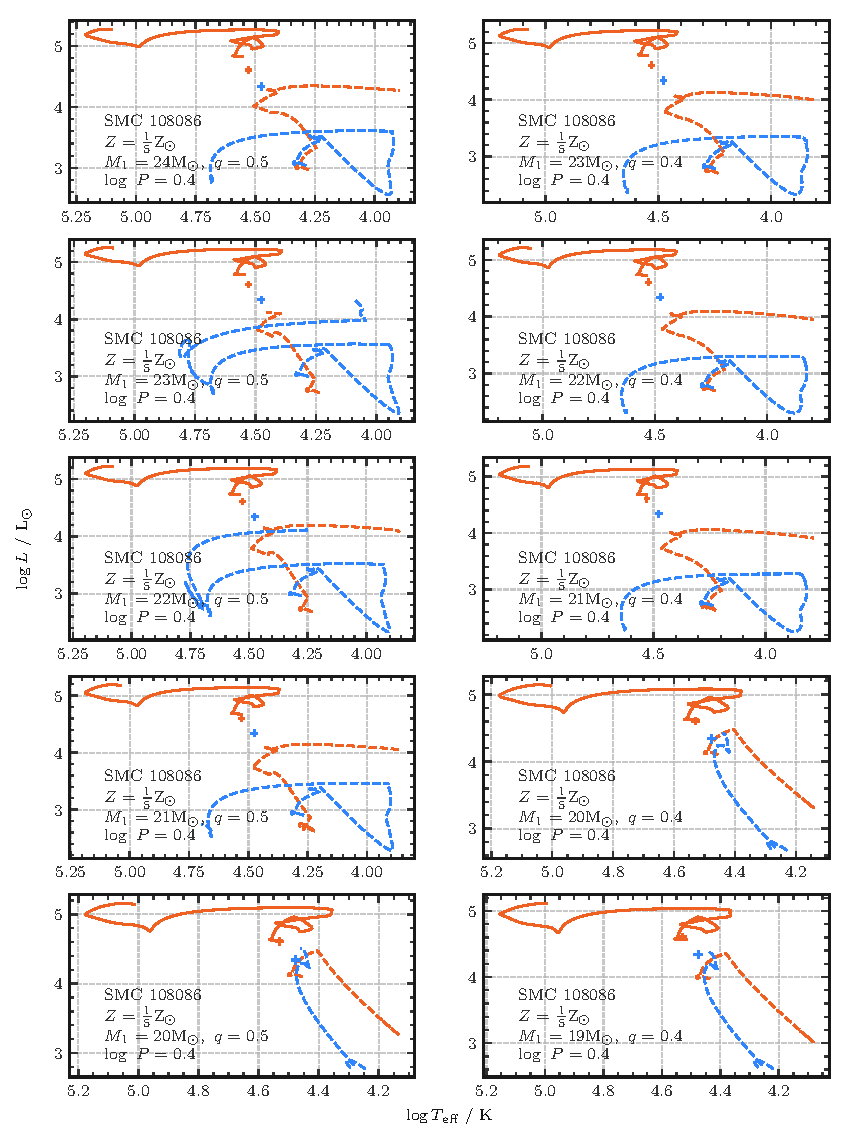
\includegraphics[width=\textwidth]{images/overcontact_binaries/bespoke_binaries/normal/SMC 108086.pdf}
        \caption{SMC 108086}
        \label{fig:bespoke_SMC_108086_normal}
    \end{subfigure}
\end{figure}%
\begin{figure}\ContinuedFloat
    \centering

    \begin{subfigure}[t]{\textwidth}
        \centering
        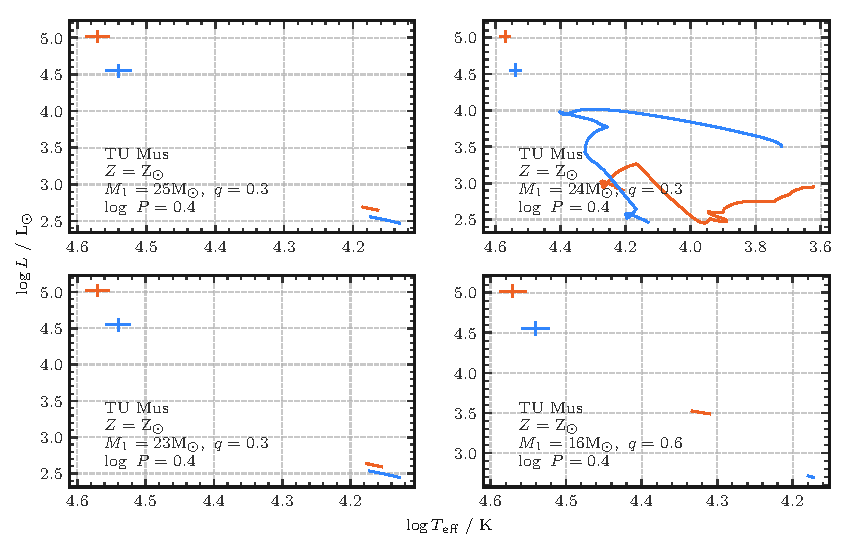
\includegraphics[width=\textwidth]{images/overcontact_binaries/bespoke_binaries/normal/TU Mus.pdf}
        \caption{TU Muscae}
        \label{fig:bespoke_TU_Mus_normal}
    \end{subfigure}

    \begin{subfigure}[t]{\textwidth}
        \centering
        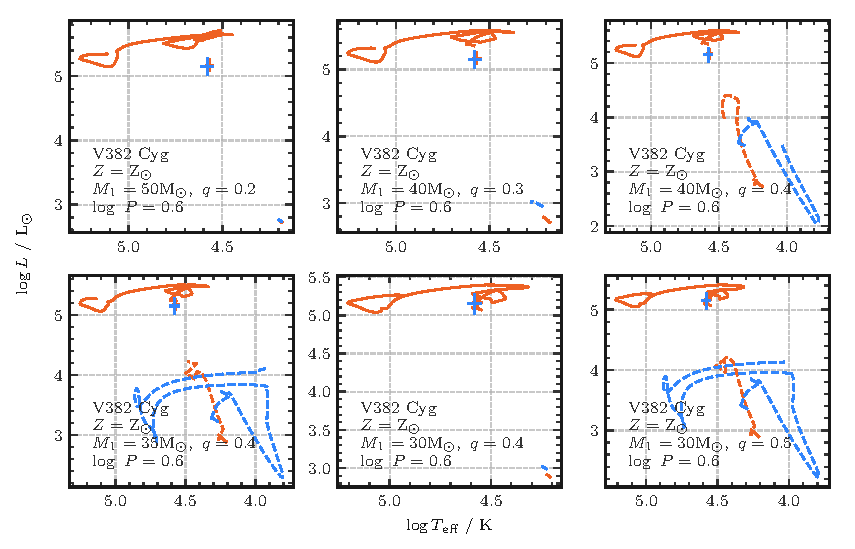
\includegraphics[width=\textwidth]{images/overcontact_binaries/bespoke_binaries/normal/V382 Cyg.pdf}
        \caption{V382 Cygni}
        \label{fig:bespoke_V382_Cyg_normal}
    \end{subfigure}

\end{figure}%
\begin{figure}\ContinuedFloat
    \centering

    \begin{subfigure}[t]{\textwidth}
        \centering
        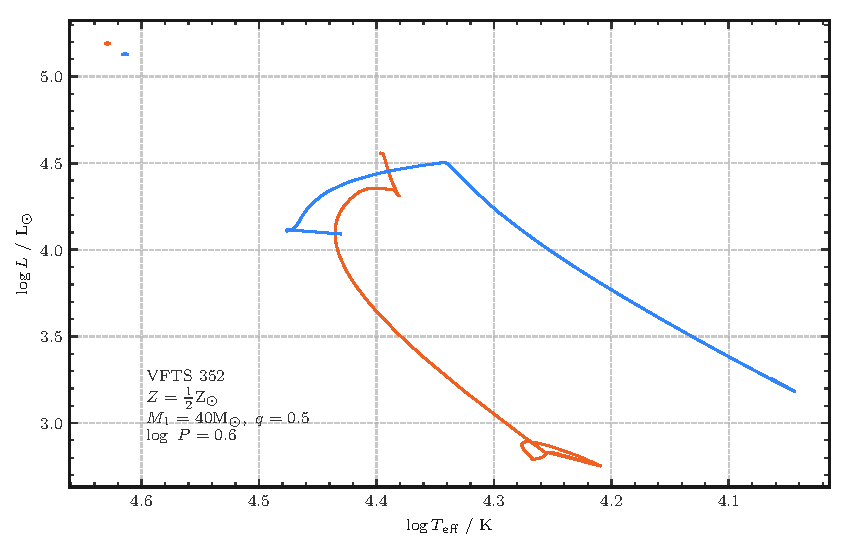
\includegraphics[width=\textwidth]{images/overcontact_binaries/bespoke_binaries/normal/VFTS 352.pdf}
        \caption{VFTS 352}
        \label{fig:bespoke_VFTS_352_normal}
    \end{subfigure}

    \caption[The results of our bespoke binary evolution for normal periods.]{The results of our bespoke binary evolution for \textbf{normal} periods. In these plots, orange lines represent the donors, and blue lines represent the accretors.}
    \label{fig:bespoke_binaries_normal}
\end{figure}
